\chapter{Περιβάλλοντα Υποβοηθούμενης Διαβίωσης}
\label{chap2}
\section{Εισαγωγή}
Τα Περιβάλλοντα Υποβοηθούμενης Διαβίωσης αποτελούν έναν αναδυόμενο διεπιστημονικό κλάδο, ο οποίος στοχεύει στην ανάπτυξη εννοιών, προϊόντων και υπηρεσιών, τα οποία θα συνδυάσουν νέες τεχνολογίες με το κοινωνικό περιβάλλον, έτσι ώστε να προσφέρουν καλύτερη ποιότητα ζωής, ειδικά σε όσα άτομα χρήζουν υποστήριξης, όπως οι ηλικιωμένοι.
Ο κλάδος βασίζεται στους τομείς της Βιοϊατρικής, του \en{Internet of Things}, του \en{Cloud Computing}, της Μηχανικής Μάθησης και πολλών άλλων.
\par
Η συνεχιζόμενη αύξηση του προσδόκιμου ζωής στην Δύση αποτελεί μια από τις μεγαλύτερες αιτίες ανάπτυξης του κλάδου.
Πλέον, απαιτούνται καινοτόμες και αποδοτικές λύσεις, με ιδιαίτερη έμφαση στην πρόληψη, για την υποστήριξη αυτών των ευαίσθητων κοινωνικών ομάδων.
Συγκεκριμένα, ο σκοπός των ΠΥΔ είναι να δημιουργήσει οφέλη για τα \textit{άτομα}, μέσω των αυξημένων δυνατοτήτων και ασφάλειας, την \textit{οικονομία}, μέσω του περιορισμού του κόστους των υπηρεσιών υγείας και τέλος την \textit{κοινωνία}, μέσω της βελτίωσης της συνολικής ποιότητας ζωής. Μια σχηματική απεικόνιση των πλεονεκτημάτων αυτών φαίνεται στο Σχήμα \ref{aalpro}. 

\section{Χαρακτηριστικά}
Δεν υπάρχει ακριβής και καθολικά αναγνωρισμένος ορισμός για τα ΠΥΔ από τους διάφορους ερευνητές των παραπλήσιων κλάδων.
Ωστόσο, μελετώντας τις διάφορες προσπάθειες ορισμού και περιγραφής τους, καταλήγουμε στον εξής ορισμό:
\begin{quote}
    Τα Περιβάλλοντα Υποβοηθούμενης Διαβίωσης αποτελούν σύγχρονες τεχνολογικές λύσεις Πληροφορικής και Επικοινωνιών, βασισμένα στις αρχές του νοήμονος περιβάλλοντος, για την παροχή καθολικής, μη επεμβατικής και προληπτικής φροντίδας σε ηλικωμένους και σε άλλα άτομα που χρήζουν φροντίδα, με τελικό σκοπό την διατήρηση της ανεξαρτησίας και την βελτίωση της ποιότητας ζωής τους, καθώς και την υποστήριξη των ατόμων που τους φροντίζουν. 
\end{quote}

\begin{figure}[h!]
\centering
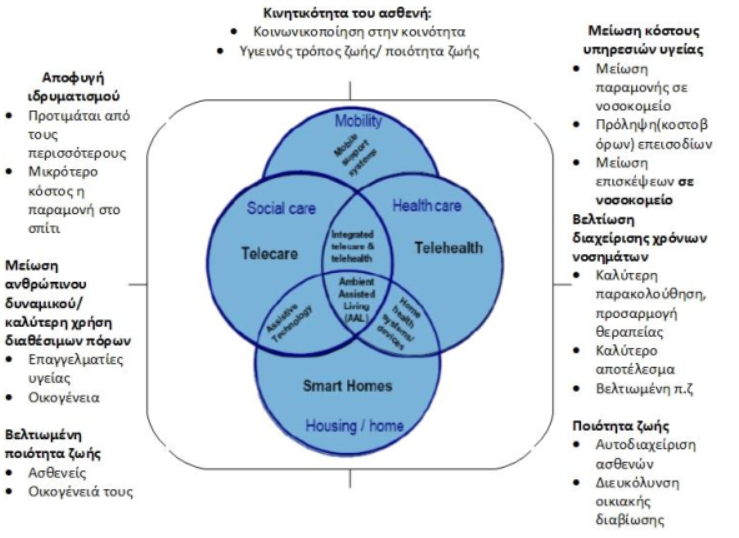
\includegraphics[scale=0.9]{images/aal.png}
\caption{Σχηματική απεικόνιση των πλεονεκτήματων των ΠΥΔ}.
\label{aalpro}
\end{figure}

Παρακάτω, θα επεξηγηθούν οι έννοιες που απαρτίζουν αυτόν τον ορισμό.

\subsection{Νοήμων περιβάλλον}
Νοήμων περιβάλλον ονομάζεται το ερευνητικό παράδειγμα, το οποίο αποδίδει υπολογιστική ευφυΐα στα καθημερινά περιβάλλοντα, μέσω της χρήσης του \en{IoT}, της διάχυτης υπολογιστικής και της τεχνητής νοημοσύνης.
Με αυτόν τον τρόπο, το ανθρωπογενές περιβάλλον μπορεί πλέον να αντιλαμβάνεται, να προσαρμόζεται και να αντιδρά στις ανάγκες μας \cite{Aarts2003}.
Τα ΠΥΔ εφαρμόζουν τις βασικές αρχές του παραδείγματος του νοήμονος περιβάλλοντος, για την δημιουργία μιας νέας γενιάς υποβοηθητικών τεχνολογιών για τους ηλικιωμένους, οι οποίες θα έχουν τα εξής χαρακτηριστικά \cite{Acampora2013}\cite{Blackman2016}:
\begin{itemize}
    \item Μη επεμβατική και απρόσκοπτη ενσωμάτωση στο περιβάλλον του χρήστη.
    \item Δράση ανάλογα με το εκάστοτε πλαίσιο και την κατάσταση του χρήστη. 
    \item Προσωποποιημένη φροντίδα για τις ανάγκες κάθε χρήστη. 
    \item Προσαρμογή στον χρήστη μέσω συνεχούς μάθησης.
    \item Προνόηση και πρόβλεψη των αναγκών και επιθυμιών του χρήστή.
\end{itemize}

Συνολικά, τα ΠΥΔ μπορούν να ειδωθούν ως το αποτέλεσμα της προόδου από τις διάφορες μεμονωμένες συσκευές, οι οποίες εξυπηρετούσαν ένα συγκεκριμένο έργο, σε ένα νοήμων περιβάλλον το οποίο θα βοηθά και υποστηρίζει τον χρήστη και τον ζωτικό του χώρο \cite{Blackman2016}.

\subsection{Σύγχρονες υπολογιστικές και επικοινωνιακές τεχνολογίες}
Τα ΠΥΔ περιλαμβάνουν ένα ευρύ φάσμα εξελιγμένων τεχνολογιών με ιδιαίτερη έμφαση στα 'έξυπνα' σπίτια, τα κινητά και ένδυτα συστήματα και την υποβοηθητική ρομποτική.\cite{rashidi2012survey}
Οι τεχνολογίες αυτές συνδυάζονται με εξελιγμένες υπολογιστικές τεχνικές, όπως η αναγνώριση ανθρώπινης δραστηριότητας, η ανακάλυψη συμπεριφορικών μοτίβων, η ανίχνευση μη ομαλών δεδομένων, η μοντελοποίηση πλαισίου, η αναγνώριση τοποθεσίας και ταυτότητας, κλπ. \cite{rashidi2012survey} \cite{Acampora2013}.
\par
Όλα τα συστατικά των ΠΥΔ είναι διασυνδεδεμένα και επικοινωνούν μεταξύ τους.
Οι ενσωματωμένοι αισθητήρες συλλέγουν πληροφορίες σχετικά με το περιβάλλον και τον χρήστη.
Οι υπολογιστικές τεχνικές συναθροίζουν την πληροφορία από τους επιμέρους αισθητήρες, την αναλύουν, την ερμηνεύουν και αποφασίζουν για την κατάλληλη δράση.
Τέλος, οι διάφοροι ενεργοποιητές, έξυπνες διεπαφές και υποβοηθητικές συσκευές δρουν αναλόγως και επιτρέπουν την διάδραση με τον χρήστη \cite{broek}.
\subsection{Η ανεξαρτησία και η βελτίωση της ποιότητας ζωής των ηλικιωμένων ως σκοπός}
Το όραμα των ΠΥΔ είναι να παρέχει στους ηλικιωμένους ασφαλή και υποστηρικτικά περιβάλλοντα , να διατηρούν και να βελτιώνουν την φυσική, πνευματική και ψυχική τους υγεία και να ενισχύουν την κοινωνική ενασχόληση και την ενεργή συμμετοχή στην κοινωνία \cite{Queiros2013}\cite{Blackman2016}\cite{broek}\cite{Peek2014}\cite{cardinaux}.
Ο απώτερος σκοπός των ΠΥΔ είναι η διασφάλιση της ανεξαρτησίας των ηλικιωμένων και η βελτίωση της ποιότητας ζωής τους.
\par
Ταυτόχρονα, η τεχνολογία των ΠΥΔ απευθύνεται και στους παρόχους φροντίδας, είτε πρόκειται για ιατρικό προσωπικό είτε για τον κοινωνικό κύκλο των ηλικιωμένων ατόμων.
Η τεχνολογία των ΠΥΔ σκοπεύει να μειώσει το βάρος των ευθυνών των παροχών φροντίδας, να ενισχύσει το αίσθημα της σιγουριάς, να βοηθήσει στην διαχείριση και τον συντονισμό των καθηκόντων φροντίδας και, τέλος, να διευκολύνει την απομακρυσμένη επικοινωνία και την κοινωνική διασύνδεση μεταξύ των παροχών φροντίδας και των ηλικιωμένων \cite{rashidi2012survey}\cite{Bossen2013}\cite{Cornejo2012}.
\section{Τομείς εφαρμογής}
Το όραμα της τεχνολογίας των ΠΥΔ αναφέρεται σε μια καθολική υποστήριξη των χρηστών. Επομένως, τα ΠΥΔ έχουν εφαρμογή σε κάθε όψη της ζωής του χρήστη.
Συγκεκριμένα, έχουν εντοπιστεί 3 βασικοί τομείς εφαρμογής, όπως παρουσιάζονται παρακάτω \cite{broek}.

\subsection{Ευγηρία στο σπίτι}
Ο πρώτος τομέας περιγράφεται ως \textit{"η δυνατότητα υγιέστερης και ποιοτικότερης καθημερινότητας, για περισσότερο χρόνο, διατηρώντας υψηλό βαθμό ανεξαρτησίας, αυτονομίας και αξιοπρέπειας"} \cite{broek}.
Η πλειοψηφία των ηλικιωμένων προτιμά την παραμονή στο γνωστό οικιακό τους περιβάλλον για το μεγαλύτερο δυνατό διάστημα \cite{Mosca2016}.
Ωστόσο, η μείωση των πνευματικών και σωματικών ικανοτήτων τους, λόγω της γήρανσης του οργανισμού, καθιστά την αυτόνομη διαμονή τους περίπλοκη και απαιτητική.
Ακόμα και ηλικιωμένοι, οι οποίοι είναι υγιείς και ενεργοί, είναι πιθανό να χρειαστούν κάποια μορφή φροντίδας στο άμεσο μέλλον.
Η δημιουργία ενός ασφαλούς και υποβοηθητικού οικιακού περιβάλλοντος είναι, επομένως, ένας σημαντικός τομέας ενδιαφέροντος των ΠΥΔ.
Παραδείγματα εφαρμογών σε αυτόν τον τομέα περιλαμβάνουν:
\begin{itemize}
    \item Οικιακά συστήματα ασφαλείας
    \item Συστήματα ελέγχου περιβαλλοντικών συνθηκών
    \item Συστήματα οικιακού αυτοματισμού
    \item Συστήματα απομακρυσμένης παρακολούθησης βιομετρικών στοιχείων
    \item Συστήματα διαχείρισης φαρμακευτικών αγωγών
    \item Συστήματα απομακρυσμένης παρακολούθησης δραστηριότητας (μοτίβα ύπνου, δίαιτας, κίνησης)
    \item Συστήματα για την αναγνώριση πτώσεων και άλλων επειγόντων περιστατικών
    \item Συστήματα υπενθύμισης και υποβοήθησης σχεδιασμού
    \item Συστήματα υποβοήθησης ατόμων με αισθητήριες αδυναμίες
    \item Ηλεκτρονικά παιχνίδια μάθησης και επικοινωνίας για ενίσχυση των πνευματικών και φυσικών ικανοτήτων
    \item Συστήματα διαχείρισης φροντίδας για την υποστήριξη των παροχέων φροντίδας
\end{itemize}{}

\subsection{Ευγηρία στην κοινότητα}

Ο δεύτερος τομέας περιγράφεται ως \textit{"η δυνατότητα κοινωνικής ενεργοποίησής και δημιουργικότητας καθημερινότητας, μέσω τεχνολογιών πληροφορικής και επικοινωνιών, προσανατολισμένες στην κοινωνική διασύνδεση και την εύκολη πρόσβαση σε δημόσιες και εμπορικές υπηρεσίες, με σκοπό την βελτίωση της ποιότητας ζωής του ατόμου και την μείωση της κοινωνικής απομόνωσης"} \cite{broek}.
Υπάρχουν αρκετοί παράγοντες που οδηγούν στην κοινωνική απομόνωση και την μοναξιά στην τρίτη ηλικία, όπως η επιδείνωση της σωματικής και ψυχικής υγείας, η αλλαγή του κοινωνικού περιβάλλοντος λόγω συνταξιοδότησης, μετακόμισης ή απώλειας συντρόφου, η ανάγκη παροχή φροντίδας σε έναν σύντροφο με προβλήματα υγείας, η έλλειψη μεταφορικού μέσου, κλπ. \cite{Wherton2009}.
\par
Η διατήρηση των κοινωνικών δεσμών και η ενεργή συμμετοχή στην κοινότητα αποτελούν κομβικά μέρη του σχεδιασμού για την \textit{ενεργή γήρανση} του Παγκόσμιου Οργανισμού Υγείας \cite{WHO2015}.
Όντως, έρευνες έχουν δείξει ότι οι κοινωνικές σχέσεις και η ενεργή κοινωνική συμμετοχή είναι σημαντικές στην ποιότητα ζωής των ηλικιωμένων ατόμων \cite{Bowling2003}\cite{GABRIEL2004}.
Η κοινωνική δικτύωση είναι συσχετισμένη με καλή φυσική, πνευματική και ψυχική υγεία \cite{Luanaigh2008}\cite{Shankar2011}\cite{Thurston2009}.
Πολλές εφαρμογές των ΠΥΔ αποσκοπούν στην μείωση της κοινωνικής απομόνωσης και στην διευκόλυνση των κοινωνικών σχέσεων και της ενεργής συμμετοχής στην κοινότητα.
Παραδείγματα εφαρμογών σε αυτόν τον τομέα περιλαμβάνουν:
\begin{itemize}
    \item Συστήματα υποβοήθησης κινητικότητας και πλοήγησης
    \item Ρομποτικά συστήματα κοινωνικής συντροφιάς
    \item Πλατφόρμες κοινωνικής δικτύωσης, επικοινωνίας και παροχής υπηρεσιών
    \item Διαδραστικά παιχνίδια και αφηγηματικά μέσα
    \item Συστήματα που διευκολύνουν την κοινωνική διάδραση και τις δράσεις αναψυχής
\end{itemize}{}

\subsection{Ευγηρία στην εργασία}
Ο τρίτος τομέας περιγράφεται ως \textit{"η δυνατότητα διατήρησης της ενεργητικότητας και της παραγωγικότητας, για ένα μεγαλύτερο χρονικό διάστημα, μέσω εύκολα προσβάσιμων και προσαρμόσιμων τεχνολογιών πληροφορικής, οι οποίες θα διευκολύνουν την δια βίου μάθηση, με σκοπό καλύτερη ποιότητα εργασίας και ισορροπία μεταξύ του χρόνου εργασίας και ιδιωτικής ζωής"} \cite{broek}.
Πάγια στρατηγική θέση της Ευρωπαϊκής Ένωσης είναι η προώθηση της παραμονής στην εργασία για μεγαλύτερο χρονικό διάστημα, για την ελάττωσή του κόστους ασφάλισης και συνταξιοδότησης του εργατικού προσωπικού \cite{morschhauser2006healthy}\cite{dubois2019extending}.
Επομένως, προκύπτει η ανάγκη για ασφαλή και υποβοηθητικά περιβάλλοντα εργασίας, τα οποία θα προωθούν την ισότητα, την υγεία και την ευημερία των γηραιότερων εργαζόμενων.
Παραδείγματα εφαρμογών σε αυτόν τον τομέα περιλαμβάνουν:
\begin{itemize}
    \item Έξυπνοι και προσαρμόσιμοι σταθμοί εργασίας
    \item Πολυτροπικές διεπαφές
    \item Συστήματα παρακολούθησης της υγείας στην εργασία
    \item Ρομποτικά συστήματα υποβοήθησης
\end{itemize}{}
\section{Εργαλεία και Τεχνικές}
Τα ΠΥΔ εκμεταλλεύονται τις εξελίξεις σε διάφορες σύγχρονες τεχνολογίες, με ιδιαίτερη έμφαση στην τεχνολογία 'έξυπνων' σπιτιών, στην κινητή και ένδυτη τεχνολογία και στην υποβοηθητική ρομποτική. Άλλες συχνά χρησιμοποιήσιμες τεχνολογίες είναι τα συστήματα διαχείρισης φροντίδας, τα συστήματα σχεδιασμού, εφαρμογές κοινωνικής δικτύωσης και επικοινωνίας, συστήματα επίγνωσης περιβάλλοντος και πλαισίου καθώς και παιχνίδια εκμάθησης και επικοινωνίας \cite{rashidi2012survey}.
Η αξιοποίησή και κατανόηση των δεδομένων, που λαμβάνονται από το περιβάλλον και τον χρήστη, απαιτεί την χρήση διάφορων εξειδικευμένων αλγορίθμων, λόγω του μεγάλου όγκου τους.
\subsection{Τεχνολογία 'έξυπνων' σπιτιών}
'Έξυπνο' σπίτι ονομάζεται ένα σπίτι το οποίο είναι εξοπλισμένο με ένα δίκτυο από διάφορους αισθητήρες και ενεργοποιητές, το οποίο συλλέγει συνεχής και συγκυριακή πληροφορία σχετικά με το οικιακό περιβάλλον και τον κάτοικο.
Στο πλαίσιο των ΠΥΔ, αυτή η πληροφορία συσσωρεύεται και χρησιμοποιείται για την παροχή ενός ασφαλούς και υποβοηθητικού οικιακού περιβάλλοντος \cite{rashidi2012survey}\cite{Liu2016}\cite{Demiris2008}.
Στον Πίνακα \ref{tab:sens} παρατίθενται διάφορα είδη αισθητήρων, τα οποία χρησιμοποιούνται συχνά στα οικιακά ΠΥΔ.

\begin{table}[h!]
    \small
    \centering
    \begin{tabularx}{\textwidth}{X X}
        Είδος Αισθητήρα&Χρήση
        \\
        \hline
         \rule{0pt}{5ex}Περιβαλλοντικοί αισθητήρες(φώς, θερμοκρασία, υγρασία, ποιότητα αέρα, κλπ) &\rule{0pt}{5ex}Άνεση, Υγιεινό περιβάλλον, Παρακολούθηση δραστηριότητας
         \\
         \rule{0pt}{5ex}Αισθητήρες καπνού και φυσικού αερίου &\rule{0pt}{5ex}Ασφάλεια
         \\
         \rule{0pt}{5ex}Αισθητήρες νερού &\rule{0pt}{5ex}Παρακολούθηση υγείας και δραστηριότητας
         \\
         \rule{0pt}{5ex}Αισθητήρες σε οικιακές συσκευές&\rule{0pt}{5ex}Άνεση, Ασφάλεια, Υποβοήθηση καθημερινών λειτουργιών, Παρακολούθηση δραστηριότητας
         \\
         \rule{0pt}{5ex}Αισθητήρες κίνησης(ενεργού και παθητικοί αισθητήρες υπερύθρων, κλπ)&\rule{0pt}{5ex}Άνεση, Ασφάλεια, Παρακολούθηση δραστηριότητας, Αναγνώριση πτώσεων και επειγόντων περιστατικών
         \\
         \rule{0pt}{5ex}Μαγνητικοί αισθητήρες σε πόρτες και παράθυρα&\rule{0pt}{5ex}Ασφάλεια, Παρακολούθηση δραστηριότητας
         \\
         \rule{0pt}{5ex}Αισθητήρες πίεσης (ενσωματωμένοι στο πάτωμα και στα έπιπλα&\rule{0pt}{5ex}Αναγνώριση πτώσεων και επειγόντων περιστατικών, Παρακολούθηση δραστηριότητας
         \\
         \rule{0pt}{5ex}\en{RFID}&\rule{0pt}{5ex}Ασφάλεια, Παρακολούθηση δραστηριότητας, Διαχείριση φαρμακευτικής αγωγής
         \\
         \rule{0pt}{5ex}Μικρόφωνο&\rule{0pt}{5ex}Αναγνώριση πτώσεων και επειγόντων περιστατικών, Παρακολούθηση δραστηριότητας
         \\
         \rule{0pt}{5ex}Κάμερα&\rule{0pt}{5ex}Ασφάλεια, Αναγνώριση πτώσεων και επειγόντων περιστατικών, Παρακολούθηση δραστηριότητας και υγείας
    \end{tabularx}
    \caption{Αισθητήρες που χρησιμοποιούνται συχνά στα οικιακά ΠΥΔ \cite{cardinaux}\cite{rashidi2012survey}}
    \label{tab:sens}
\end{table}

\par
Στην διάρκεια των τελευταίων 2 δεκαετιών, έχουν αναπτυχθεί διάφορα προγράμματα "έξυπνων" σπιτιών.
Ένα από αυτά είναι το πρόγραμμα "\en{Aware Home}" στις ΗΠΑ. Πρόκειται για ένα τριώροφο σπίτι, το οποίο είναι εξοπλισμένο με μια ποικιλία από αισθητήρες (κάμερες, μικρόφωνα, \en{RFID}, αισθητήρες πίεσης,  κλπ.) \cite{aware_home}.
Οι αισθητήρες διακριτικά παρακολουθούν και υποστηρίζουν τους κατοίκους.
Οι εφαρμογές τους περιλαμβάνουν ένα δίκτυο αισθητήρων πίεσης ενσωματωμένο στο πάτωμα, το οποίο είναι σε θέση να εντοπίσει και να αναγνωρίσει τους κατοίκους, ένα μνημονικό βοήθημα βασισμένο σε αισθητήρες \en{RFID}, το οποίο βοηθάει τους κατοίκους να βρίσκουν χαμένα αντικείμενα και ένα σύστημα συνολικής παρακολούθησης και επικοινωνίας, το οποίο παρέχει πληροφορίες για τις καθημερινές δραστηριότητες των κατοίκων σε απομακρυσμένους συγγενείς.
\par
Στην Ευρώπη, το ερευνητικό πρόγραμμα \en{ENABLE} ανέπτυξε και δοκίμασε αρκετές τεχνολογίες για την υποστήριξη ατόμων με ήπια έως μέτρια άνοια στο Ηνωμένο Βασίλειο, την Ιρλανδία, την Νορβηγία, την Φινλανδία και την Λιθουανία \cite{Adlam2004}\cite{Cahill2007}.
Οι τεχνολογικές λύσεις που αναπτύχθηκαν περιλαμβάνουν ένα δίκτυο αισθητήρων στις οικιακές συσκευές της κουζίνας, το οποίο φρόντιζε για την ασφαλή χρήση τους (π.χ. κλείσιμο φούρνου ύστερα από ορισμένη ώρα), καθώς και ένα σύστημα εντοπισμού της νυχτερινής δραστηριότητας και την αυτόματη ενεργοποίηση του απαραίτητου φωτισμού. 
\par
Άλλα γνωστά παραδείγματα εφαρμογών 'έξυπνων' σπιτιών περιλαμβάνουν τα προγράμματα: \en{Casas} \cite{Cook2013}, \en{MavHome} \cite{Das2004}, \en{Ubiquitous Home} \cite{yamazaki2007}, \en{Glouchester Smart House} \cite{Orpwood2004} και το \en{Future Care Lab} \cite{Klack2011}.

\subsection{Κινητή και ένδυτη τεχνολογία}
Η πρόοδος στην επιστήμη υλικών και την μικροηλεκτρονική έχει επιτρέψει την ανάπτυξη ολοένα και μικρότερων, πιο εύκαμπτων και φθηνότερων αισθητήρων.
Αυτή η συνεχιζόμενη αλλαγή στους διαθέσιμους αισθητήρες, έχει εφοδιάσει με ισχυρά εργαλεία τους τομείς της απομακρυσμένης παρακολούθησης της υγείας και της δραστηριότητας των ηλικιωμένων ατόμων, όπως φαίνεται και στο Σχήμα \ref{wearable}.
Οι τομείς αυτοί, έχουν σκοπό την υποστήριξη της διαχείρισης της υγείας και της αποκατάστασης της στο οικιακό περιβάλλον των ασθενών, μέσω της συνεχής παρακολούθησης των φυσιολογικών δεικτών, της καταγραφής της τοποθεσίας και της κίνησης και της αναγνώρισης και ανάλυσης των μοτίβων δραστηριότητας.
\begin{figure}[h!]
\centering
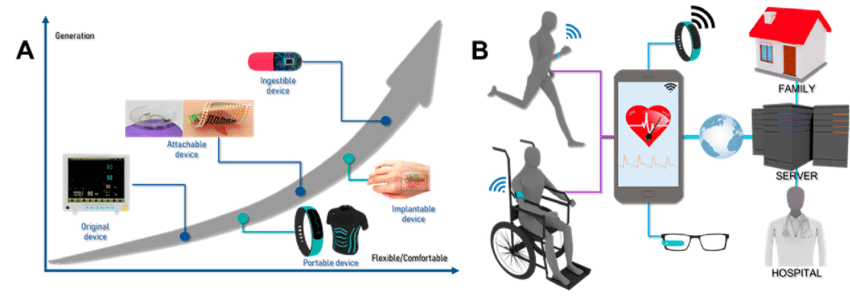
\includegraphics[scale=0.5]{images/wearable.png}
\caption{Σχηματική απεικόνιση των διάφορων εργαλείων της ένδυτης τεχνολογίας}.
\label{wearable}
\end{figure}

\subsubsection{'Έξυπνα' κινητά και ρολόγια}
Τα 'έξυπνα' κινητά (\en{smartphones}) είναι εξοπλισμένα με διάφορους αισθητήρες, όπως επιταχυνσιόμετρο, γυροσκόπιο, αισθητήρες εγγύτητας, \en{GPS}, \en{Bluetooth}, φωτογραφική μηχανή, μικρόφωνο και αισθητήρες περιβαλλοντικών συνθηκών, οι οποίοι μπορούν να αξιοποιηθούν για παρακολούθηση δραστηριότητας σε εσωτερικούς και εξωτερικούς χώρους \cite{Incel2013}.
Τα 'έξυπνα' ρολόγια (\en{smartwatches}) έχουν επίσης χρησιμοποιηθεί για παρακολούθηση δραστηριότητας, καθώς είναι εξοπλισμένα με παρόμοιους αισθητήρες \cite{Chernbumroong2011}\cite{Sen2015}.
\par
Σε αντίθεση με τα \en{smartphones}, οι περιβραχιόνιες συσκευές είναι πιο αξιόπιστες στην αναγνώριση δραστηριοτήτων που περιλαμβάνουν κινήσεις χεριών, όπως η κατανάλωση φαγητού, ποτού ή το κάπνισμα \cite{Shoaib2016} .
Επίσης, παρέχουν συνεχή δεδομένα για την παρακολούθηση σε εσωτερικούς χώρους, καθώς μπορούν να φορεθούν άνετα 24 ώρες την ημέρα \cite{Bieber2013}\cite{Rawassizadeh2014}.
Τα \en{smartphones} έχουν καλύτερες επιδόσεις στην αναγνώριση των υπόλοιπων δραστηριοτήτων, διότι το μεγαλύτερο χρονικό διάστημα βρίσκονται κοντά στην λεκάνη, οπότε και είναι κατάλληλα για την αναγνώρισή δραστηριοτήτων, όπως η ποδηλασία ή το τρέξιμο \cite{Shoaib2016}\cite{Bieber2013}.
Πρόσφατες μελέτες προσπάθησαν να συνδυάσουν τα δεδομένα των αισθητήρων και από τις 2 συσκευές για προχωρημένη αναγνώριση δραστηριότητας \cite{Shoaib2016}\cite{Casilari2015}.
\par
Τα \en{smartwatches} και, συνολικά, οι περιβραχιόνιες συσκευές, λόγω της τοποθέτησης τους και της συνεχής επαφής τους με το δέρμα, είναι κατάλληλες για την παρακολούθηση φυσιολογικών δεικτών, όπως ο καρδιακός ρυθμός (μέσω του ηλεκτροκαρδιογραφήματος (\en{ECG}) ή του φωτοπληθυσμιογραφήματος (\en{PPG}) ), την θερμοκρασία του σώματος, την εφίδρωση (μέσω της ηλεκτροδερματικής δραστηριότητας \en{GSR}) και της μυϊκής δραστηριότητας (μέσω της ηλεκτρομυογραφήματος (\en{EMG}) \cite{Rawassizadeh2014}\cite{Klonovs2016}.
\par
Αρκετές έρευνες έχουν χρησιμοποιήσει \en{smartphones}, \en{smartwatches} και άλλες περιβραχιόνιες 
συσκευές στον τομέα των ΠΥΔ.
Συγκεκριμένα, έχουν χρησιμοποιηθεί διαθέσιμα στην αγορά \en{smartphones} και \en{smartwatches} για την αναγνώριση πτώσεων ηλικιωμένων ατόμων.
Η χρήση αυτών των συσκευών μείωσε τον αριθμό των λανθασμένων συναγερμών, ενώ ταυτόχρονα βελτίωσε την ικανότητα ανίχνευσης πραγματικών πτώσεων \cite{Casilari2015}.
Σε άλλες έρευνες, η αξιοποίηση των δεδομένων από τις συγκεκριμένες συσκευές απέτρεψε την αφυδάτωση ηλικιωμένων ατόμων μέσω της παρακολούθησης των κινήσεων των χεριών τους \cite{Lutze2015}.

\subsubsection{'Έξυπνα' ρούχα και υφάσματα}
Τα 'έξυπνα' ρούχα και υφάσματα προσφέρουν άλλο ένα εργαλείο για μη επεμβατική παρακολούθηση της υγείας και της δραστηριότητας των ατόμων.
Έχουν αναπτυχθεί αισθητήρες που μπορούν να ενσωματωθούν στα ρούχα, στο ύφασμα και στις ίνες του υφάσματος \cite{rashidi2012survey}.
Ένα παράδειγμα ενός 'έξυπνου' ρούχου είναι το γιλέκο \en{MagIC}.
Το συγκεκριμένο γιλέκο διαθέτει πλεκτά ηλεκτρόδια για καταγραφή ηλεκτροκαρδιογραφήματος (\en{ECG}), έναν υφασμάτινο αισθητήρα πληθυσμιογραφήματος για την παρακολούθηση του αναπνευστικού ρυθμού και ένα επιταχυνσιόμετρο.
Χρησιμοποιήθηκε για την απομακρυσμένη παρακολούθηση καρδιοπαθών \cite{Rienzo2010}.
\par
Ένα παρόμοιο ρούχο είναι το \en{t-shirt} \en{Smart Vest}.\cite{Pandian2008}
Περιέχει αισθητήρες ενσωματωμένους στο ύφασμα, οι οποίοι συλλέγουν διάφορους φυσιολογικούς δείκτες, όπως το ηλεκτροκαρδιογράφημα (\en{ECG}), το φωτοπληθυσμιογράφημα για την μέτρηση της ροής και πιέσης του αίματος (\en{PPG}), την θερμοκρασία του σώματος, την εφίδρωση μέσω του \en{GSR}, αλλά και την τοποθεσία μέσω \en{GPS}.
Ταυτόχρονα, γίνονται έρευνες \cite{Chang2013} για να αναπτυχθούν υφασμάτινοι χωρητικοί αισθητήρες σε διάφορα σημεία του σώματος, με σκοπό την καταγραφή διάφορων φυσιολογικών δεικτών, όπως το ηλεκτροκαρδιογράφημα και ο ρυθμός αναπνοής, οι κινήσεις του καρπού και του χεριού, η κατανάλωση φαγητού και ποτού καθώς και πληροφορίες για το βάδισμα του ατόμου.
\par
Υπάρχουν και άλλες δημοφιλείς ένδυτες συσκευές, οι οποίες, συνήθως, επισυνάπτονται στα παπούτσια, στη ζώνη ή στα κοσμήματα του χρήστη \cite{Brodie2016}\cite{Achkar2016}\cite{Sardini2010}\cite{Sim2011}.
\subsubsection{Επιδερμικά ηλεκτρονικά συστήματα}
Ένα ακόμη αισθητηριακό εργαλείο για την καταγραφή της υγείας είναι αισθητήρες ενσωματωμένοι σε επιφάνειες, οι οποίες είναι συνημμένες στο δέρμα. 
Ωστόσο, η συγκεκριμένη λύση έχει περιορισμένη περιθώρια αξιοποίησης στην καθημερινή ζωή, καθώς δεν είναι εύχρηστη και οι αισθητήρες μπορούν εύκολα να αποσπαστούν από το δέρμα \cite{Yeo2013}.
Πρόσφατα, αναπτύχθηκαν εύκαμπτες και λεπτές μεμβράνες, οι οποίες ονομάζονται επιδερμικά ηλεκτρονικά συστήματα.
Οι ιδιότητες τους επιτρέπουν μια πιο σταθερή και στενή διεπαφή της μεμβράνης με το δέρμα, επιτρέποντας την συνεχή και σταθερή καταγραφή φυσιολογικών μετρήσεων \cite{Imani2016}.
Αν και τα περισσότερα παρόμοια συστήματα συλλέγουν φυσικές ή ηλεκτροφυσιολογικές παραμέτρους, όπως το ηλεκτροκαρδιογράφημα ή η θερμοκρασία του δέρματος \cite{Bian2014}\cite{Webb2013}\cite{Yeo2013}, υπάρχουν ορισμένα τα οποία συλλέγουν και βιοχημικές παραμέτρους, όπως η συγκέντρωση γαλακτικού οξέος στον ιδρώτα \cite{Imani2016}.
\subsubsection{Ενδοσωματικά συστήματα}
Μια πιο επεμβατική λύση για την παρακολούθηση της υγείας ενός χρήστη είναι τα συστήματα που εισέρχονται στο σώμα του.
Παραδείγματα τέτοιων λύσεων είναι αισθητήρες γλυκόζης, οι οποίοι εισέρχονται υποδόρια για την ανίχνευση υπογλυκαιμίας στο αίμα \cite{Juhl2010}.
και κάψουλες, οι οποίες χορηγούνται από το στόμα, και καταγράφουν την θερμοκρασία, την πίεση, εικόνες και το \en{pH} στο εσωτερικό του σώματος \cite{McCaffrey2008}.
\subsection{Υποβοηθητική ρομποτική}
Η υποβοηθητική ρομποτική στα ΠΥΔ χωρίζεται στις εξής 3 ευρείς κατηγορίες, τα ρομπότ ανάρρωσης και παροχής φροντίδας, τα κοινωνικά ρομπότ παροχής υπηρεσιών και τα ρομπότ συντροφιάς, όπως φαίνεται και στο Σχήμα \ref{robot_start} \cite{Broekens2009}\cite{Robinson2014}.
\begin{figure}[h!]
\centering
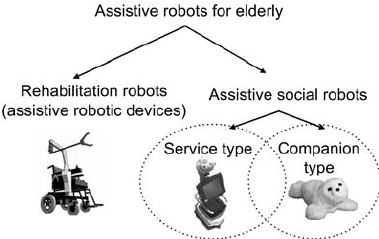
\includegraphics[scale=0.6]{images/robotics_start.png}
\caption{Σχηματική απεικόνιση των κατηγοριών της υποβοηθητικής ρομποτικής}.
\label{robot_start}
\end{figure}
Η πρώτη κατηγορία περιγράφεται ως "συσκευές οι οποίες βοηθάνε φυσικά τον χρήστη χωρίς να έχουν κύριο σκοπό την επικοινωνία ή να μπορούν να θεωρηθούν κοινωνικές οντότητες" \cite{Robinson2014}.
Τα ρομπότ ανάρρωσης βοηθούν στην φυσική εξάσκηση, συνεισφέρουν στην διαχείριση μειωμένων φυσικών
ικανοτήτων και βοηθούν τους ηλικιωμένους στις καθημερινές δραστηριότητες τους.
Παραδείγματα που ανήκουν σε αυτήν την κατηγορία είναι ρομπότ υποβοήθησης κίνησης \cite{Spenko2006}, εξωσκελετοί \cite{OSullivan2015} και ρομπότ που βοηθούν με την φυσική εξάσκηση και αποκατάσταση \cite{Johnson2006}.
\par
Η δεύτερη κατηγορία είναι τα κοινωνικά ρομπότ παροχής υπηρεσιών.
Ο σκοπός τους είναι να βοηθούν τους ηλικιωμένους στις διάφορες δραστηριότητες της καθημερινότητας, να βοηθούν στις μετακινήσεις τους και να παρακολουθούν την υγεία και ασφάλεια τους.
Τα συγκεκριμένα ρομπότ χαρακτηρίζονται ως κοινωνικά διότι μπορούν να αλληλεπιδράσουν άμεσα με τους ηλικιωμένους \cite{Robinson2014}.
Το ρομπότ \en{Pearl} είναι ένα ανθρωποειδές κοινωνικό ρομπότ παροχής υπηρεσιών, το οποίο έχει ύψος 1 μέτρο, και αλληλεπιδρά με τον χρήστη μέσω ομιλίας, οθονών, εκφράσεις του προσώπου και φυσική κίνηση \cite{Pineau2003}\cite{Pollack2002}.
Σχεδιάστηκε για να βοηθά ηλικιωμένους, μέσω της υπενθύμισης και της οργάνωσης διάφορων καθημερινών εργασιών και δραστηριοτήτων, όπως τα γεύματα, η φαρμακευτική αγωγή και η πλοήγηση στο περιβάλλον τους.
\par
Το ρομπότ \en{Care-o-bot} ανήκει στην ίδια κατηγορία \cite{Hans2002}\cite{Kittman2015}\cite{Reiser2013}.
Η τελευταία εκδοχή του είναι ανθρωπόμορφη και έχει ύψος 1.5 μέτρο.
Σε σχέση με τις προηγούμενες εκδοχές του, έχει δοθεί προσοχή στα μέσα αλληλεπίδρασης και στην φυσικότητα του σώματος του, για την βελτίωση της κοινωνικότητας του.
Ο χρήστης μπορεί να αλληλεπιδράσει μαζί του μέσω χειρονομιών, ομιλίας, οθόνης αφής και εφαρμογής σε κινητό.
Το \en{Care-o-bot} μπορεί να αντιδράσει με εκφράσεις του προσώπου, κινήσεις των χεριών και του σώματος καθώς και με τα ενσωματωμένα ηχεία του.
Με τα εύκαμπτα χέρια του μπορεί να μεταφέρει και να χειριστεί αντικείμενα \cite{Kittman2015}.
Άλλα παραδείγματα ρομπότ παροχής υπηρεσιών είναι το \en{RIBA} \cite{Mukai2010} και το \en{Kompa}{\"i} \cite{Kompai2017}.
\par
Η τρίτη κατηγορία είναι τα ρομπότ συντροφιάς.
Κυρία λειτουργία τους είναι η ενίσχυση της συναισθηματικής ευμάρειας και η μείωση της μοναξιάς, παρέχοντας συντροφιά και διευκολύνοντας τις κοινωνικές αλληλεπιδράσεις \cite{Broekens2009}.
Ένα παράδειγμα ρομπότ συντροφιάς είναι ο \en{Paro}, μια ρομποτική φώκια καλυμμένη με μαλακή γούνα.
O \en{Paro} αντιδρά στην ομιλία, στο να τον χαϊδεύουν και να τον κρατάνε, κουνώντας το κεφάλι και τα πτερύγια του, ανοιγοκλείνοντας τα μάτια του και μιμούμενος την φωνή μιας νεαρής φώκιας.
Σκοπός του είναι να προκαλέσει αντίστοιχα συναισθήματα με ένα πραγματικό κατοικίδιο, ώστε να μειωθεί το άγχος και η ανησυχία, προσφέροντας ψυχολογική παρηγοριά και τονώνοντας τις κοινωνικές επαφές \cite{Wada2005}.
\par
Ένα ακόμα ρομπότ συντροφιάς είναι ο \en{AIBO}, ένας κινητός ρομποτικός σκύλος με ενσωματωμένους αισθητήρες και ένα σκληρό πλαστικό εξωτερικό.
Ο \en{AIBO} μπορεί να κουνήσει το κεφάλι, την ουρά και τα πόδια του.
Έχει δοκιμαστεί σε περιβάλλοντα με ηλικιωμένους και έρευνες έδειξαν πως μειώνει το άγχος και την μοναξιά και ενισχύει την κοινωνική συμπεριφορά \cite{Kanamori2002}\cite{Tamura2004}.
Ο \en{Zora} είναι ένα ανθρωποειδές ρομπότ συντροφιάς, το οποίο στοχεύει να ενεργοποιήσει και να αλληλεπιδράσει με τους ηλικιωμένους, τραγουδώντας, χορεύοντας ή ενθαρρύνοντας φυσική εξάσκηση \cite{Helianthe2017}\cite{Melkas2016}\cite{Parviainen2016}.
\par
Τα τελευταία χρόνια, ο διαχωρισμός μεταξύ των 3 κατηγοριών γίνεται ολοένα και πιο ασαφής, καθώς οι κατασκευαστές ρομπότ υπηρεσίας περιλαμβάνουν περισσότερα κοινωνικά μέσα και μέσα αλληλεπίδρασης, για να αυξήσουν την αποδοχή των χρηστών.
Επομένως, είναι πιθανό τα μελλοντικά ρομπότ να παρέχουν και αυξημένη λειτουργική υποστήριξη αλλά και κοινωνική συντροφιά.
\begin{figure}[h!]
\centering
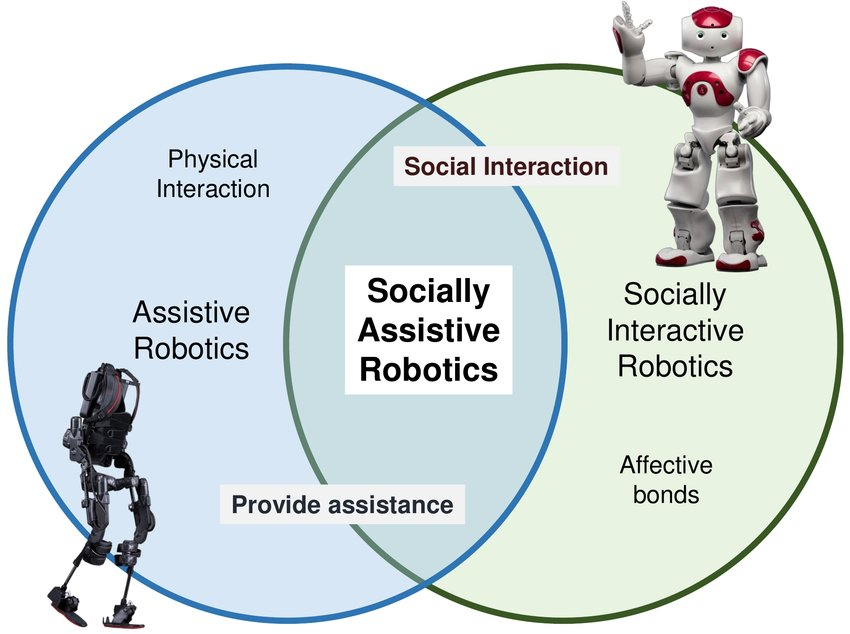
\includegraphics[scale=1]{images/robotics_end.jpg}
\caption{Σχηματική απεικόνιση των σκοπών της υποβοηθητικής ρομποτικής}.
\label{robot_end}
\end{figure}
\subsection{Αλγόριθμοι και υπολογιστικές τεχνικές}
Ο μεγάλος όγκος και ποικιλία των δεδομένων που συλλέγονται από τις διάφορες εφαρμογές των ΠΥΔ απαιτούν ειδικούς αλγορίθμους και υπολογιστικές τεχνικές για την κατανόηση και διαχείριση τους.
Παρακάτω θα παρουσιάσουμε μια περίληψη των πιο συχνών τεχνικών που χρησιμοποιούνται στις εφαρμογές των ΠΥΔ.

\subsubsection{Αναγνώριση δραστηριότητας}
Τα ΠΥΔ χρειάζονται να αναγνωρίσουν τι κάνουν οι χρήστες τους, βασισμένα σε μια ποικιλία δεδομένων, για να παρέχουν προληπτική βοήθεια.
Σημαντικές δραστηρίοτητες περιλαμβάνουν τον ύπνο, το περπάτημα, την εξάσκηση, την κατανάλωση φαγητού και ποτού και την λήψη της φαρμακευτικής αγωγής.
Η προσέγγιση για την αναγνώριση δραστηριότητας εξαρτάται από τους υποκείμενους αισθητήρες, τον αλγόριθμο μηχανικής μάθησης που μοντελοποιεί την δραστηριότητα και την πολυπλοκότητα της δραστηριότητας προς μάθηση.
\subsubsection{Αναγνώριση συμπεριφορικών μοτίβων}
Μια σχετική προσέγγιση είναι η αναγνώριση επαναλαμβανόμενων μοτίβων στα συγκεντρωμένα δεδομένα δραστηριότητας, μέσω τεχνικών μάθησης χωρίς επιτήρηση.
Τα μοτίβα αυτά συνεισφέρουν στην κατανόηση και ερμηνεία των δεδομένων που συλλέγονται από τους αισθητήρες και μπορούν να χρησιμοποιηθούν για την κατασκευή νέων μοντέλων για την αναγνώριση των μοτίβων αυτών στο μέλλον.
\subsubsection{Αναγνώριση ανωμαλιών}
Η αναγνώριση ανωμαλιών αναφέρεται στον εντοπισμό μοτίβων στα συγκεντρωμένα δεδομένα, τα οποία αποκλίνουν από την αναμενόμενη συμπεριφορά.
Αυτό είναι κομβικό για τα ΠΥΔ, για να μπορέσει να αναγνωρίσει αλλαγές στην καθημερινή ρουτίνα, μη συμμόρφωση με την φαρμακευτική αγωγή, πτώσεις ή άλλες επείγοντες καταστάσεις.
Η αναγνώριση ανωμαλιών είναι πιο ακριβής με συμπεριφορές, οι οποίες πραγματοποιούνται σε τακτική βάση.
\subsubsection{Μοντελοποίηση πλαισίου}
Τα συστήματα ΠΥΔ πρέπει να προσαρμόζονται σε δυναμικές πληροφορίες πλαισίου, σχετικά με το φυσικό περιβάλλον, τον χρήστη και το υπολογιστικό υπόβαθρο \cite{Bettini2010}.
Επομένως, τα συστήματα πρέπει να μπορούν να αναπαραστήσουν την συναφή πληροφορία, όπως η χωρική πληροφορία του περιβάλλοντος, το ιατρικό ιστορικό, το προφίλ και τις προτιμήσεις του χρήστη, την πληροφορία για τους υπάρχοντες αισθητήρες.
\subsubsection{Σχεδιασμός και οργάνωση}
Ο αυτοματοποιήμενος σχεδιασμός και οργάνωση μπορούν να έχουν μεγάλη αξία σε διάφορες ΠΥΔ εφαρμογές.
Παραδείγματα περιλαμβάνουν την υπενθύμιση των απαραίτητων δραστηριοτήτων σε άτομα με πνευματικές βλάβες και την αυτοματοποίηση της καθημερινής ρουτίνας ατόμων με φυσικά προβλήματα.
\subsubsection{Αναγνώριση ταυτότητας και τοποθεσίας}
Η ανάγκη για παρακολούθηση, ανίχνευση και παροχή προληπτικής και φυσικής βοήθειας στους χρήστες, εξυπηρετείται στα ΠΥΔ από συστήματα ταυτοποίησης και εντοπισμού των ηλικιωμένων ειδικά σε κατοικίες με πολλούς κατοίκους.

\section{Προκλήσεις}
Υπάρχουν αρκετές προκλήσεις στον τομέα των ΠΥΔ που δεν έχουν λυθεί ακόμα, παρά τις υποσχόμενες τεχνικές εξελίξεις.
\subsection{Τεχνική υλοποίηση}
Τα έξυπνα σπίτια και οι ένδυτες συσκευές συλλέγουν έναν πολύ μεγάλο όγκο δεδομένων.
Αυτά είναι η βάση της προσωποποιημένης, προληπτικής και περιβάλλουσας βοήθειας, ωστόσο συνεπάγονται σοβαρά ζητήματα ασφάλειας και ιδιωτικότητας.
Απαιτείται η χρήση πρωτοκόλλων ασφαλείας και η χρήση ειδικών τεχνικών προστασίας δεδομένων.
Αυτό είναι ιδιαίτερα σημαντικό για ευαίσθητα δεδομένα, όπως ιατρικά δεδομένα ή οπτικό υλικό.
Ο συνδυασμός των διάφορων διασυνδεδεμένων αισθητήρων και συσκευών περαιτέρω δυσχεραίνει την υλοποίηση ασφαλούς ανάλυσης και αποθήκευσης δεδομένων \cite{Acampora2013}\cite{Ghayvat2015}\cite{rashidi2012survey}.
Η διαλειτουργικότητα και η τυποποίηση των αισθητήρων και συσκευών, προκειμένου να μπορούν να επικοινωνήσουν μεταξύ τους, είναι ένα επιπλέον πρόβλημα το οποίο προσπαθούν να λύσουν οι ερευνητές \cite{Memon2014}\cite{Queiros2013}.
Επίσης, ένα συνολικό πρόβλημα που αντιμετωπίζουν τα ΠΥΔ είναι ο σχεδιασμός απλών και διαισθητικών διεπαφών, ώστε να διευκολυνθεί η φυσική αλληλεπίδραση με τα ηλικιωμένα άτομα \cite{Queiros2013}\cite{Sun2009}.
\par
Ένα ακόμα πρόβλημα των συστημάτων ΠΥΔ είναι η αξιοπιστία.
Η αξιόπιστη αναγνώριση της δραστηριότητας και της συμπεριφοράς του χρήστη σε ένα μη ελεγχόμενο και μη οικιακό περιβάλλον, όπως το οικιακό, είναι ένα απαιτητικό πρόβλημα.
Πολλές έρευνες αναφέρουν προβλήματα αξιοπιστίας, όπως λάθος συναγερμοί, χαμηλή ακρίβεια πρόβλεψης ή αδυναμία διαχείρισης πολλαπλών χρηστών, παρά την συνεχή εξέλιξη των αλγορίθμων και των αισθητήρων.
Τα ζητήματα αξιοπιστίας δεν οδηγούν μόνο σε δυσφορία και μειωμένη εμπιστοσύνη μεταξύ των χρηστών, αλλά μπορούν να έχουν σοβαρές επιπτώσεις στην υγεία και την ευμάρεια τους.
Επομένως, η βελτίωση της αξιοπιστίας των ΠΥΔ παραμένει κομβικό ζήτημα προς επίλυση \cite{Liu2016}\cite{rashidi2012survey}\cite{cardinaux}.
\par
Στην περίπτωση των ένδυτων λύσεων, υπάρχει η επιπλέον πρόκληση να σχεδιαστεί μια άνετη, ελαφριά και ασφαλής συσκευή με καλή αισθητική, σχεδιασμό και χαμηλή ενεργειακή κατανάλωση, ώστε να μπορεί και θέλει ο χρήστης να την φοράει 24 ώρες την μέρα.
Ταυτόχρονα, οι προγραμματιστές και οι σχεδιαστές αυτών των συσκευών χρειάζεται να ενσωματώσουν σε αυτές, το απαραίτητο υλικό και λογισμικό για αξιόπιστη, ασφαλή και συνεχή συλλογή δεδομένων \cite{Ghayvat2015}.
\par
Αντίστοιχα, η μεγαλύτερη πρόκληση της υποβοηθητικής ρομποτικής είναι η διευκόλυνση της φυσικής αλληλεπίδρασης και κοινωνικής σύμπλεξης μεταξύ ρομπότ και ηλικιωμένων.
Οι ερευνητές συνεχίζουν να δουλεύουν προς μια αποδεκτή φυσική εμφάνιση, τον σχεδιασμό χειρονομιών, εκφράσεων προσώπου και σωματικών κινήσεων που να προσεγγίζουν τις ανθρώπινες και την δημιουργία κοινωνικής νοημοσύνης και αυτόνομης συμπεριφοράς \cite{Robinson2014}\cite{Mataric2017}.
Επιπλέον, τα περισσότερα ρομπότ έχουν περιορισμένη λειτουργικότητα και δεν είναι σε θέση να βοηθήσουν σε πολλές και περίπλοκες δραστηριότητες της καθημερινότητας \cite{rashidi2012survey}.
Μια ακόμα ανησυχία για την υποβοηθητική ρομποτική είναι η εγγυημένη ασφαλής κίνηση και λειτουργία σε ένα οικιακό περιβάλλον \cite{Salem2015}.
\par
Πρόσφατες συστηματικές έρευνες\cite{Liu2016}\cite{Memon2014} ανέδειξαν ότι, παρά την εκτενή έρευνα στον τομέα,  η συνολική τεχνολογική ετοιμότητα των ΠΥΔ εφαρμογών είναι ακόμα χαμηλή, οι περισσότερες εφαρμογές μένουν σε πιλοτικό στάδιο και λίγες από αυτές καταλήγουν σε προϊόν.
Ορισμένα από τα βασικά εμπόδια για την υλοποίηση και διάδοση των ΠΥΔ συστημάτων είναι η αβεβαιότητα του κόστους τους και η έλλειψη κανονισμών και ρυθμίσεων σχετικά με τον διαμοιρασμό και αποζημίωση του κόστους τους από τους αντίστοιχους ασφαλιστικούς φορείς \cite{rashidi2012survey}\cite{Reeder2013}\cite{Vimarlund2014}.
Ωστόσο, σύγχρονες έρευνες άρχισαν να προσεγγίζουν τα παραπάνω προβλήματα, αναλύοντας την αποδοτικότητα των συστημάτων ΠΥΔ με όρους κόστους και εξερευνώντας τρόπους να συνδέσουν τα ΠΥΔ συστήματα με τα διάφορα συστήματα υγείας \cite{Manetti2017}.
\subsection{Αποδοχή από τους χρήστες}
Η πιο σημαντική συνθήκη για την διάδοση των ΠΥΔ είναι η αποδοχή των χρηστών.
Αρκετές συστηματικές ανασκοπήσεις αναδεικνύουν την αποδοχή αυτή ως ένα από τα μεγάλα εμπόδια για την υλοποίηση και διάδοση των ΠΥΔ συστημάτων σε πραγματικές συνθήκες \cite{Peek2014}\cite{rashidi2012survey}\cite{Robinson2014}.
Όντως, η φύση και ο σκοπός των ΠΥΔ έχουν σημαντικές επιπτώσεις στην αποδοχή από τους χρήστες.
Αυτές οι συσκευές καταλαμβάνουν ιδιωτικό χώρο είτε στο οικιακό περιβάλλον είτε ακόμα και πάνω στο σώμα των χρηστών, συλλέγουν και αποθηκεύουν προσωπικά και ιατρικά δεδομένα, επηρεάζουν την συμπεριφορά και τις συνήθειες, ωθούν τους χρήστες τους να κοινωνικοποιηθούν μέσω ή με μια μηχανή και αναλαμβάνουν εργασίες οι οποίες προορίζονται για άνθρωπο, είτε τον ίδιο τον χρήστη ή κάποιο πάροχο φροντίδας.
\par
Η αποδοχή των χρηστών, λοιπόν, απασχολεί όλο και περισσότερες έρευνες \cite{Liu2016}.
Ωστόσο, ο τομέας παραμένει κινούμενος με γνώμονα την τεχνολογία και όχι τον χρήστη, καθώς οι ερευνητές και σχεδιαστές ΠΥΔ εφαρμογών δεν έχουν σαν προτεραιότητα την κάλυψη των αναγκών των χρηστών \cite{Queiros2013}.
Αυτό οδηγεί σε στερεοτυπικές συμπεριφορές, υπεραπλούστευση και ανεπαρκής κατανόηση των αναγκών του χρήστη, τα οποία συνεπώς, οδηγούν σε κακό σχεδιασμό και υλοποίηση προϊόντων τα οποία τείνουν να απορρίπτονται από τους χρήστες \cite{Eisma2004}\cite{Ostlund2005}\cite{Peine2014}\cite{Vines2015}.
\par
Επομένως, οι ηλικιωμένοι και οι πάροχοι υγείας πρέπει να εμπλακούν στην διαδικασία σχεδιασμού και ανάπτυξης έτσι ώστε να αποφευχθεί ένα κενό μεταξύ των αναγκών των χρηστών και τις πεποιθήσεις των ερευνητών \cite{rashidi2012survey}\cite{Piau2013}\cite{Queiros2013}.
Επιπλέον, ο κλάδος οφείλει να αναπτύξει μια περιεκτική κατανόηση, βασισμένη στην θεωρία, τον παραγόντων αυτών που προωθούν ή αποθαρρύνουν την αποδοχή των ΠΥΔ.
Τα συμπεράσματα αυτά μπορούν να αξιοποιηθούν στις διαδικασίες σχεδιασμού και ανάπτυξης νέων προϊόντων, αυξάνοντας έτσι την πιθανότητα αποδοχής τους από τους μελλοντικούς τους χρήστες.
\subsection{Εφαρμογές μεγάλης κλίμακας και θεωρητικός διάλογος}
Οι περισσότερες έρευνες σχετικά με τα ΠΥΔ υποστηρίζουν ότι οι τεχνολογίες αυτές έχουν την δυνατότητα υποστήριξης μιας υγιούς και αυτόνομης γήρανσης για τους ηλικιωμένους, ωστόσο οι κλινικές ενδείξεις είναι λίγες και αδύναμες.
Οι \en{Demiris} και \en{Hensel} δεν βρήκαν καμία έρευνα οι οποία να παρουσιάζει θετικές ενδείξεις για την επίδραση των ΠΥΔ στην βελτίωση της υγείας, στην αντιμετώπιση επειγόντων περιστατικών ή στην αποφυγή περίθαλψης σε γηροκομείο \cite{Demiris2008}.
Ο \en{Liu} βρήκε ορισμένες έρευνες που παρουσιάζουν υποσχόμενες κλινικές ενδείξεις για την χρήση των ΠΥΔ στην παρακολούθηση των καθημερινών δραστηριοτήτων, της μείωσης των πνευματικών δυνατοτήτων, της ψυχικής υγείας και καρδιολογικών παθήσεων \cite{Liu2016}.
Οι ερευνητές δεν βρήκαν κάποια μελέτη που να παρουσιάζει κλινικά στοιχεία για την πρόβλεψη αναπηρίας, την αποφυγή πτώσεων και την βελτίωση της ποιότητας ζωής των χρηστών.
Ο \en{Robinson} κατέληξε ότι η υποβοηθητική ρομποτική χρειάζεται περισσότερες δοκιμές σε πραγματικά οικιακά περιβάλλοντα, ώστε να αποδειχθεί η δυνατότητα προσαρμογής τους στην καθημερινότητα ηλικιωμένων ατόμων και, στη συνέχεια, αποτελεσματικής υποστήριξης τους \cite{Robinson2014}.
\par
Η δεδομένη μεθοδολογική προσέγγιση για να μετρήσουν την αποδοχή των χρηστών είναι ποιοτική και όχι ποσοτική, ενώ ο αριθμός των δειγμάτων συνήθως είναι μικρός.
Είναι απαραίτητη η διεξαγωγή μεγαλύτερης κλίμακας ερευνών για να κατανοηθεί η σχετική σημασία των παραγόντων που επηρεάζουν την αποδοχή των ΠΥΔ από τους χρήστες, η αναγνώριση των υποκείμενων σχέσεων μεταξύ τους και η εξαγωγή συμπερασμάτων για την επίδραση τους στην διαδικασία αποδοχής.
Άλλες έρευνες αναφέρουν την ανησυχία ότι ο τομέας των ΠΥΔ είναι πλούσιος σε δεδομένα και όχι σε θεωρία \cite{Blackman2016}.
Ο \en{Liu} επιβεβαιώνει αυτήν την ανησυχία, καθώς καμία από τις μελέτες σχετικά με την αποδοχή των ΠΥΔ δεν χρησιμοποίησε ένα θεωρητικό πλαίσιο για την εξήγηση και θεμελίωση των ευρημάτων τους \cite{Liu2016}.
Η ανάπτυξη ενός θεωρητικού διαλόγου θα βοηθούσε τους ερευνητές των ΠΥΔ να κατανοήσουν τους υποκείμενους κοινωνικούς, ψυχολογικούς και συμπεριφορικούς μηχανισμούς της διαδικασίας αποδοχής.
\par
Συνολικά, είναι σαφές πως υπάρχει έλλειψη αποδεδειγμένων μεθοδολογικών προσεγγίσεων, όπως τυχαία ελεγχόμενες δοκιμές, μακροχρόνιες μελέτες, ποσοτικές μελέτες μεγάλης κλίμακας και θεωρητικές προσεγγίσεις, για την κατανόηση της διάδοσης και της αποδοτικότητας των εφαρμογών ΠΥΔ \cite{Martin2008}\cite{Morris2013}\cite{Peek2014}.